\section{Augmented Reality}


\subsection {Definition}

Was ist AR?
Das Konzept der erweiterten Realität (Augmented Reality, AR) wurde von vielen Forschern der Informatik unter Berücksichtigung verschiedener Faktoren unterschiedlich definiert.

Die ersten Definitionen wurden von Milgram, Takemura, Utsumi und Kishino vorgeschlagen
(1994). In ihrer Arbeit “Augmented Reality: A class of displays on the reality-virtuality continuum” (Eine Klasse von Displays auf dem Realitäts-Virtualitäts-Kontinuum) konzeptualisierten sie das Virtual-Reality-Kontinuum, das vier Systeme berücksichtigt: reale Umgebung (Real Environment), erweiterte Realität (Augmented Reality), erweiterte Virtualität (Augmented Virtuality) und virtuelle Umgebung (Virtual Environment). Darüber hinaus wurden zwei Ansätze zur Definition von “Augmented Reality” genannt: eine breite Definition und eine präzisere Definition. In der breiten Definition wird Augmented Reality definiert als “Erweiterung des natürlichen Feedbacks an den Operator mit simulierten Hinweisen”. Im Gegensatz dazu wird sie im genaueren Verständnis definiert als “eine Form der virtuellen Realität, bei der das am Kopf montierte Display des Teilnehmers transparent ist und eine klare Sicht auf die reale Welt ermöglicht”.  \cite{Milgram94a} \cite{Milgram94b}
\vspace{1cm}
\begin{figure}[h!]
    \centering
    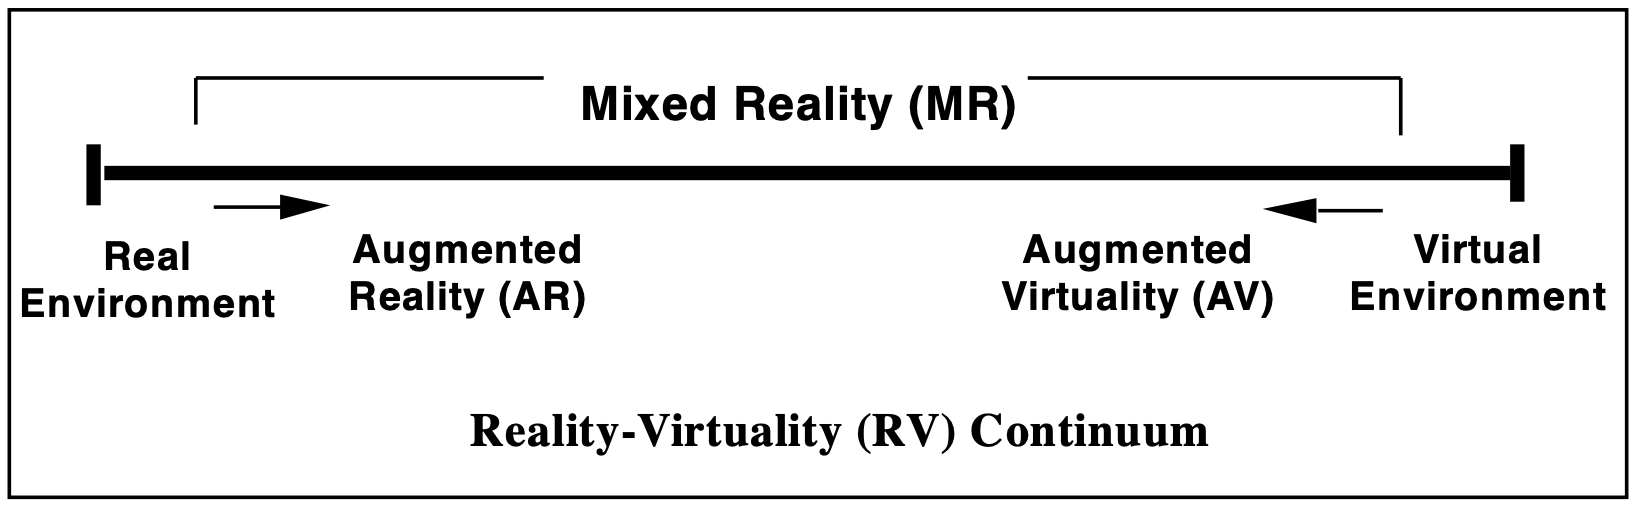
\includegraphics[width=0.9\textwidth]{attachments/MR_Definition.png}
    \caption{Vereinfachte Darstellung eines “Reality-Virtuality (RV) Continuum”.}  \cite{Milgram94a}
    \end{figure}
    

    \newpage

Andere Forscher, wie z. B. T. Azuma, definieren AR anhand seiner Merkmale oder Eigenschaften. Nach seinem Ansatz wird AR als Systeme definiert, die die folgenden drei Merkmale aufweisen:
\begin{enumerate}
    \item kombiniert reale und virtuelle Objekte in einer realen Umgebung;
    \item läuft interaktiv und in Echtzeit;
    \item registriert (richtet aus) in 3-D reale und virtuelle Objekte miteinander.  \cite{Azuma1997ASO}
\end{enumerate}


\subsection {Schlüsseltechnologien}

% An Augmented Reality System can be divided into two components: one is hardware, and the other is software  \cite{craig2013understanding}, \cite{Chatzopoulos}.
Ein Augmented-Reality-System kann in zwei Komponenten unterteilt werden: die Hardware und die Software \cite{craig2013understanding}, \cite{Chatzopoulos}.

% The main characteristic of the hardware components is to acquire and display the data and information, and process it. The \textbf{input components} are sensors that respond to physical or chemical stimuli from the real environment and provide the necessary data for the development of the system. The \textbf{output components} are devices for displaying the information, which can be divided into wearable and non-wearable, as well as optical, video, and projection devices. The output itself can be further divided into two variants of displays: \textbf{Optical See-through Display}, where the virtual contents are projected onto the interface to mix with the real scene optically, and \textbf{Video See-through Display}, which has two work modalities: one uses HMD (Head-Mounted Display) devices, and the other works with camera and screen in handheld devices, such as smartphones and tablets \cite{Azuma1997ASO}. 
Das Hauptmerkmal der Hardwarekomponenten ist die Erfassung und Anzeige der Daten und Informationen sowie deren Verarbeitung. Die \textbf{Input-Komponenten} sind Sensoren, die auf physikalische oder chemische Reize aus der realen Umgebung reagieren und die notwendigen Daten für die Entwicklung des Systems liefern. Die \textbf{Output-Komponenten} sind Geräte zur Anzeige der Informationen, die in tragbare und nicht tragbare sowie optische, Video- und Projektionsgeräte unterteilt werden können. Die Ausgabe selbst kann weiter in zwei Varianten von Displays unterteilt werden: \textbf{Optisch durchsichtiges Display (Optical See-through Display)}, bei dem die virtuellen Inhalte auf die Schnittstelle projiziert werden, um sich optisch mit der realen Szene zu vermischen, und \textbf{Video-Durchsichtiges Display (Video See-through Display)}, bei dem es zwei Arbeitsmodalitäten gibt: eine verwendet HMD-Geräte (Head-Mounted Display), die andere arbeitet mit Kamera und Bildschirm in Handheld-Geräten wie Smartphones und Tablets \cite{Azuma1997ASO}.

\newpage

\vspace{1cm}

\begin{figure}[h!]
    \centering
    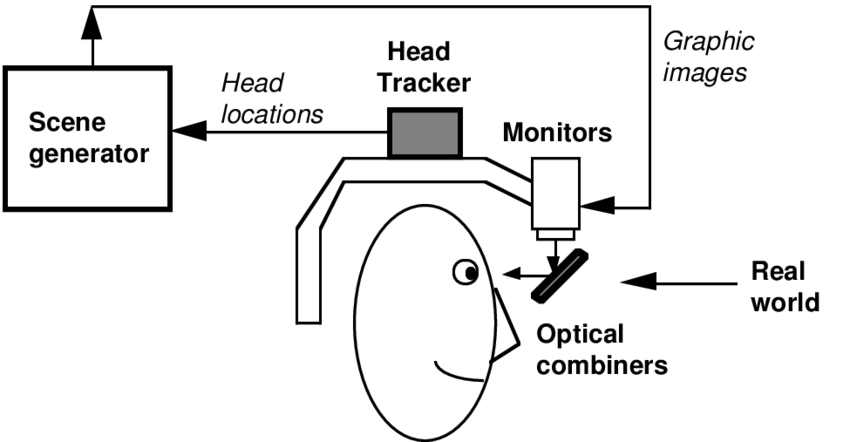
\includegraphics[width=0.65\textwidth]{attachments/Diagram_2.png}
    \caption{Optisch durchsichtiges Display}  \cite{Azuma1997ASO}
    \end{figure}

% \textbf{Video-Durchsichtiges Display (Video See-through Display):} hat zwei Arbeitsmodalitäten: Die eine verwendet HMD(Head-Mounted Display)-Geräte, die andere arbeitet mit Kamera und Bildschirm in Handheld-Geräten. Zum Beispiel Smartphones und Tablets.

\vspace{1cm}

\begin{figure}[h!]
    \centering
    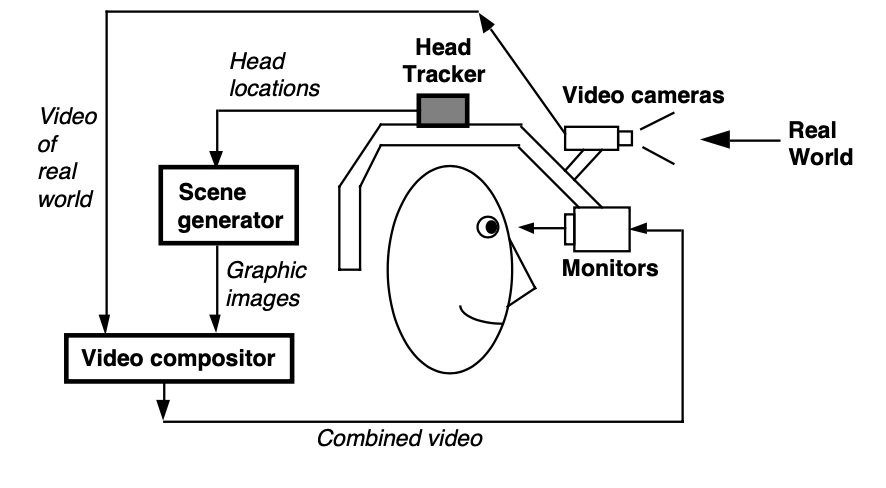
\includegraphics[width=0.75\textwidth]{attachments/Diagram_1.png}
    \caption{Video-Durchsichtiges Display}  \cite{Azuma1997ASO}
    \end{figure}

% On the software side, one of the key tasks is to derive real-world coordinates that are independent of the camera and camera images. This process is known as image registration and involves various computer vision methods, particularly those related to video tracking  \cite{Azuma2001RecentAI}.
Auf der Software-Seite besteht eine der Hauptaufgaben darin, reale Koordinaten abzuleiten, die von der Kamera und den Kamerabildern unabhängig sind. Dieser Prozess wird als Bildregistrierung bezeichnet und umfasst verschiedene Computer-Vision-Methoden, insbesondere solche, die sich auf die Videoverfolgung beziehen \cite{Azuma2001RecentAI}.